\documentclass[hidelinks]{article}
\usepackage{amsmath}
\usepackage{geometry}
\usepackage{amsfonts}
\usepackage{hyperref}
\geometry{margin=1in}
\usepackage{mathtools}
\usepackage{annotate-equations}

\usepackage{pgfplots}
\usepackage{hyperref}


\author{Derek Caughy}
\title{ECO2100 Part 2 Homework 1}
\date{November 13, 2025}
\begin{document}
\maketitle
\section*{a)}
Social welfare is given by:\\
\\
\begin{equation*}
	S=\tikzmarknode{production}{f(k)}\tikzmarknode{employed}{(1-u)}-\tikzmarknode{costs}{vk}
\end{equation*}
\annotate[yshift=1em]{left}{production}{Production of firm in match}
\annotate[yshift=0.5em]{above}{employed}{Number of matches}
\annotate[yshift=-0.5em]{below}{costs}{total cost of vacancies}\\
\\
Note that we want to solve the steady state level of unemployment. First note that\\
\\
\begin{equation*}
	\tikzmarknode{utime}{\dot{u}}=\tikzmarknode{destruction}{\delta(1-u)}-\tikzmarknode{creation}{\frac{m(\lambda)}{\lambda}u}
\end{equation*}
\annotate[yshift=0.5em]{left}{utime}{change in unemployment across time, =0 in steady state}
\annotate[yshift=-1em]{below}{destruction}{rate of job destruction times employed}
\annotate[yshift=0.5em]{right}{creation}{mathcing rate of unemployed workers times unemployed}
\\
Thus in steady state:
\[0=\delta -(\delta+\frac{m(\lambda)}{\lambda})u\]
\[\iff u=\frac{\delta}{\delta+\frac{m(\lambda)}{\lambda}}=\frac{\lambda\delta}{\lambda\delta+m(\lambda)}\]
Furthermore, note that
\[\lambda=\frac{u}{v} \iff v=\frac{u}{\lambda}=\frac{\delta}{\lambda\delta+m(\lambda)}\]
Thus we can write the social planner's problem
\begin{align*}
	\max_{\lambda\geq0, k>0} &f(k)\frac{m(\lambda)}{\lambda\delta+m(\lambda)}-k\frac{\delta}{\lambda\delta+m(\lambda)}\\
\end{align*}
The Lagrangian can be written as:
\[\mathcal{L}(\lambda, k, \mu_1, \mu_2)=\frac{f(k)m(\lambda)-k\delta}{\lambda\delta+m(\lambda)}+\mu_1(k-\epsilon)+\mu_2\lambda\]
where $\epsilon>0$ is an arbitrary constant.

\section*{b)}
First note, that $\epsilon$ is arbitrary, therefore we can always choose some $\epsilon$ such that $k>\epsilon>0$, thus by complementary slackness $\mu_1=0$. Secondly, for finite 
The first order conditions are written as follows:
\begin{align*}
	\frac{f'(k)m(\lambda)-\delta}{\lambda\delta+m(\lambda)}&=0 \tag{k}\\
	\frac{f(k)m'(\lambda)\bigl(\lambda\delta+m(\lambda)\bigr)-\bigl(\delta+m'(\lambda)\bigr)\bigl(f(k)m(\lambda)-k\delta\bigr)}{\bigl(\lambda\delta+m(\lambda)\bigr)^2}+\mu_2&=0 \tag{$\lambda$}\\
\end{align*}
Inspecting condition (k) and taking the limit as $\lambda \rightarrow 0$ reveals that $\lambda\neq 0$. That is, 
\[\lim_{\lambda\rightarrow 0}\frac{f'(k)m(\lambda)-\delta}{\lambda\delta+m(\lambda)}=\frac{-\delta}{\infty}<0\]
By complementary slackness, it follows that $\mu_2=0$
Now inspect FOC ($\lambda$) we can derive:
\[f(k)m'(\lambda)\bigl(\lambda\delta+m(\lambda)\bigr)-\bigl(\delta+m'(\lambda)\bigr)\bigl(f(k)m(\lambda)-k\delta\bigr)=0\]
by the denominator necessairily being nonzero. This can be simplified:
\[\lambda f(k)m'(\lambda)-f(k)m(\lambda)+k\bigl(\delta+m'(\lambda)\bigr)=0\]
\[\iff \bigl(\lambda m'(\lambda)-m(\lambda)\bigr)f(k)+k\bigl(\delta+m'(\lambda)\big)=0\]
\[\iff \bigl(1-\frac{\lambda m'(\lambda)}{m(\lambda)}\bigr)f(k)-k\bigl(\frac{\delta}{m(\lambda)}+\frac{m'(\lambda)}{m(\lambda)}\bigr)=0\]
Define
\[\eta(\lambda)=\frac{\lambda m'(\lambda)}{ m(\lambda)}\iff \frac{m'(\lambda)}{m(\lambda)}=\frac{\eta(\lambda)}{\lambda}\]
Then re-write the above:
\[\bigl(1-\eta(\lambda)\bigr)f(k)-k\bigl(\frac{\delta}{m(\lambda)}+\frac{\eta(\lambda)}{\lambda}\bigr)=0\]






\section*{c)}
\begin{align}
	rJ(k)&=f(k)-w-\delta\bigl(J(k)-V(k)\bigr) \label{J} \tag{i}\\
	rV(k)&=-k+m(\lambda)\bigl(J(k)-V(k)\bigr) \label{V} \tag{ii} \\
	rW(k)&=w -\delta \bigl(W(k)-U(k)\bigr) \label{W} \tag{iii} \\
	rU(k)&=\frac{m(\lambda)}{\lambda}\bigl(W(k)-U(k)\bigr) \label{U} \tag{iv}
\end{align}

\section*{d)}

First, note that by $k=\bar{k}$ that the above Bellman equations are no longer functions of k. Furthermore, the equilibrium wage rate will be given by Nash Bargaining. That is 

\[w=\arg\max_\beta (W-U)^\beta(J-V)^{(1-\beta)}\]
\[=\arg\max_\beta \beta \ln(W-U)+(1-\beta)\ln(J-V)\]
The first order condition yields:
\[\beta\frac{\frac{\partial W}{\partial w}}{W-U}+(1-\beta)\frac{\frac{\partial J}{\partial w}}{J-V}=0\]
The partial derivatives come from the fact that W and J are functions of w, while V and U are not. Re-writing \ref{W}:
\[W=\frac{w+\delta U}{r+\delta}\]
Doing the same for J in terms of \ref{J} yields:
\[J=\frac{f(k)-w+\delta V}{r+\delta}\]
It becomes obvious that $\frac{\partial W}{\partial w}=-\frac{\partial J}{\partial w}$ thus the first order condition can be re-written:
\[\beta\frac{1}{W-U}-(1-\beta)\frac{1}{J-V}=0\]
\[\iff \beta(J-V)=(1-\beta)(W-U)\]
Now we note the free entry condition which means that $V=0$ we can re-write the FOC to be:
\begin{equation*}
	\eqnmarkbox[blue]{WU}{W-U}=\beta\bigl(W-U+\eqnmarkbox[red]{J2}{J}\bigr)
\end{equation*}
\annotate[yshift=-1em]{below}{WU}{$=\frac{w-rU}{r+\delta}$ from \ref{W}}
\annotate[yshift=-1em]{below}{J2}{$=\frac{f(k)-w}{r+\delta}$ from \ref{J}}\\
\\
\[\iff \frac{w-rU}{r+\delta}=\frac{\beta}{r+\delta}(f(k)-rU)\]
\begin{equation}
	\iff w=(1-\beta)rU+\beta f(k) \label{FOC} \tag{garbage}
\end{equation}
From the FOC we can also derive:
\[W-U=\frac{\beta}{1-\beta}J\]
From \ref{V} we can obtain
\[J=\frac{k}{m(\lambda)}\]
Thus:
\[W-U=\frac{\beta}{1-\beta}\frac{k}{m(\lambda)}\]
Which can be subsititued into \ref{U} to obtain
\[rU=\frac{m(\lambda)}{\lambda}\frac{\beta}{1-\beta}\frac{k}{m(\lambda)}=\frac{\beta}{1-\beta}\frac{k}{\lambda}\]
Substituing into \ref{FOC} and doing some simplifying:
\[w=\beta \frac{k}{\lambda}+\beta f(k)\]
\[\iff w=\beta(f(k)+\frac{k}{\lambda})\]
Now inspect \ref{V} using J from \ref{J}
\[0=-k+m(\lambda)\frac{f(k)-w}{r+\delta}\]
\[\iff w=f(k)-\frac{r+\delta}{m(\lambda)}k\]
Thus
\[\beta(f(k)+\frac{k}{\lambda})=f(k)-\frac{r+\delta}{m(\lambda)}k\]
\[\iff (1-\beta) f(k)-k\bigl(\frac{\beta}{\lambda}+\frac{r+\delta}{m(\lambda)}\bigr)=0\]
Setting $r=0$ and solving for $f(k)$:
\[f(k)=\frac{1}{1-\beta} k \bigl(\frac{\beta}{\lambda}+\frac{\delta}{m(\lambda)}\bigr)\]
Now taking the First order condition for $\lambda$ from part b and solving for $f(k)$:
\[f(k)=\frac{1}{1-\eta(\lambda)}k\bigl(\frac{\delta}{m(\lambda)}+\frac{\eta(\lambda)}{\lambda}\bigr)\]
Then if the two solutions are equal we have
\[\frac{1}{1-\eta(\lambda)}\bigl(\frac{\delta}{m(\lambda)}+\frac{\eta(\lambda)}{\lambda}\bigr)=\frac{1}{1-\beta} k \bigl(\frac{\beta}{\lambda}+\frac{\delta}{m(\lambda)}\bigr)\]
\[\iff (1-\beta)\frac{\delta\lambda+\eta(\lambda)m(\lambda)}{\lambda m(\lambda)}=(1-\eta(\lambda))\frac{\delta\lambda+\beta m(\lambda)}{\lambda m(\lambda)}\]
\[\iff \beta=\eta(\lambda)\]
This is the same Hosios condition that we saw in class. The intuition is that the efficient solution depends on the elasticity of the matching function. In words, the bargining power of the firm must be equal to the elasticity of the matching function for the firm. Because both of the variables are exogenous, this is coincidental if it occurs and in general does not hold. We can view $\beta$ as a Pigouvian tax on firms that forces firms to internalize the cost of spurious entry. It's a Pigouvian tax in the sense that market entry has externalities for workers. More vacancies causes faster matching which increases the value to workers. The optimal Pigouvian tax, being equal to the elasticity of the matching rate makes intuitive sense. The elasticity of the matching function proidves a measure of the marginal costs associated with firm entry. 


\section*{e)}

%The second equilibrium condition for this economy, given that firms are allowed to choose k, would be that firms are optimally choosing k. Assume that $\bar{k}$ from the previous question is optimal. Then in equilibrium (letting $r=0$), it follows that
%\[f(k)=\frac{1}{1-\beta}k\bigl(\frac{\beta}{\lambda}+\frac{\delta}{m(\lambda)}\bigr)\]
%Taking the derivative with respect to $k$
%\[f'(k)=\frac{1}{1-\beta}\bigl(\frac{\beta}{\lambda}+\frac{\delta}{m(\lambda)}\bigr)\]
%Recall one of the first order conditions from b) that determined $k^*$ and $\lambda^*$, and solve for $f'(k)$:
%\[f'(k)=\frac{\delta}{m(\lambda)}\]

The second equilbrium condition is that firms will choose k such that they are maximizing the value of having a vacancy. That is:
\[rV(k)=-k+m(\lambda)\bigl(J(k)-\max_k V(k)\bigr)\]
It follows from the free entry condition that $\max_k V(k)=0$. Thus the firm will maximize:
\[rV(k)=-k+m(\lambda)J(k)\]
Note that from \ref{J} that
\[J(k)=\frac{f(k)}{r+\delta}-\frac{w}{r+\delta}\]
Thus
\[rV=-k+m(\lambda)\bigl(\frac{f(k)}{r+\delta}-\frac{w}{r+\delta}\bigr)\]
Recall from the previous part that $w=\beta\bigl(f(k)-\frac{k}{\lambda}\bigr)$ then,
\[rV(k)=-k+\frac{m(\lambda)}{r+\delta}\bigl(f(k)-\beta \bigl(f(k)+\frac{k}{\lambda}\bigr)\bigr)\]
\[=(1-\beta)\frac{m(\lambda)}{r+\delta}f(k)-k(1+\beta\frac{m(\lambda)}{\lambda(r+\delta)})\]
Yields the following the first order condition:
\[(1-\beta)\frac{m(\lambda)}{r+\delta}f'(k)-(1+\beta\frac{m(\lambda)}{\lambda(r+\delta)})=0\]
Taking $r=0$ we have:
\[f'(k)=\frac{\delta}{(1-\beta)m(\lambda)}+\frac{\beta}{1-\beta}\frac{1}{\lambda}\]
Note that if the market level of k is equal to the optimal level of capital we require (from the FOC derived in part b))
\[\frac{\delta}{(1-\beta)m(\lambda)}+\frac{\beta}{1-\beta}\frac{1}{\lambda}=\frac{\delta}{m(\lambda)}\]
\[\iff \beta=0\]

It follows that the market equilibrium and planner's solution will only have the same level of $k$ if $\beta=0$. This corresponds to the firms extracting all surplus of production. My best guess at the intuition would be that if firms are required to split surplus with the workers, they will underproduce compared to the efficient level of production. That is, the social planner simply maximized production subject to market frictions, while firms will maximize production minus wages subject to market frictions. The introduction of non-zero wages deters firms from entry. Figure \ref{trash} attempts to visualize this. The basic condition for firm profit maximization is expected marginal revenue, captured by $f'(k)$ is equal to expected marginal cost, captured by $w+k$. In the social planner's problem this marginal costs is simply $k$. This is obviously abstracting from the fact that firms only face costs of production in terms of k when not producing, but hopefully the intuition still holds. Even though firms do not face capital costs when operating, firms still maximize their expected value which includes expectations over when firms have vacancies. 

\begin{figure}[ht]
	\centering
	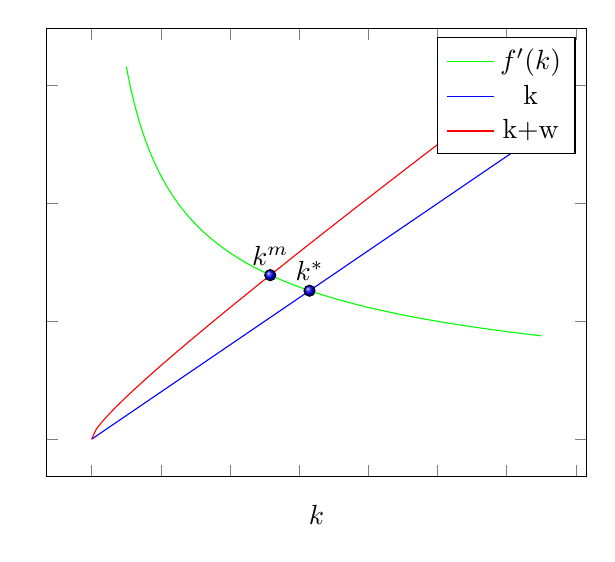
\begin{tikzpicture}
		\begin{axis}[xlabel=$k$, yticklabel=\empty, xticklabel=\empty]
			\addplot[domain=0.1:1.3, samples=100, color=green]{1/2/sqrt(x)};
			\addlegendentry{$f'(k)$}
			\addplot[domain=0:1.3, samples=5, color=blue]{x};
			\addlegendentry{k}
			\addplot[domain=0:1.3, samples=100, color=red]{x+0.25*sqrt(x)};
			\addlegendentry{k+w}
			\addplot [only marks, mark=ball, point meta=explicit symbolic, nodes near coords] coordinates {(0.51626,0.6958) [$k^{m}$] (0.6299,0.6299) [$k^*$]};


		\end{axis}
		
	\end{tikzpicture}
	\caption{A really trash graph}
	\label{trash}
\end{figure}

\section*{f)}

From the two efficiency conditions derived from parts d) and e) together imply that this economy will never be efficient. The two conditions on $\beta$ are disjoint.  Recall that the two joint conditions imply
\[0=\beta=\eta(\lambda)=\frac{\lambda m'(\lambda)}{m(\lambda)}\neq0\]
Equilibrium $\lambda$ will only ever be efficient for a strictly positive bargaining power for workers, while the condition for k states that production will only ever be efficient when workers have no bargaining power. The incentives for efficient $\lambda$ and efficient k do not align for the firm. Worker bargaining power is required to keep firms from spuriously entering the market, however positive bargaining power also adds costs to production which lowers k. 







\end{document}